% Created by tikzDevice version 0.10.1 on 2018-01-23 02:20:48
% !TEX encoding = UTF-8 Unicode
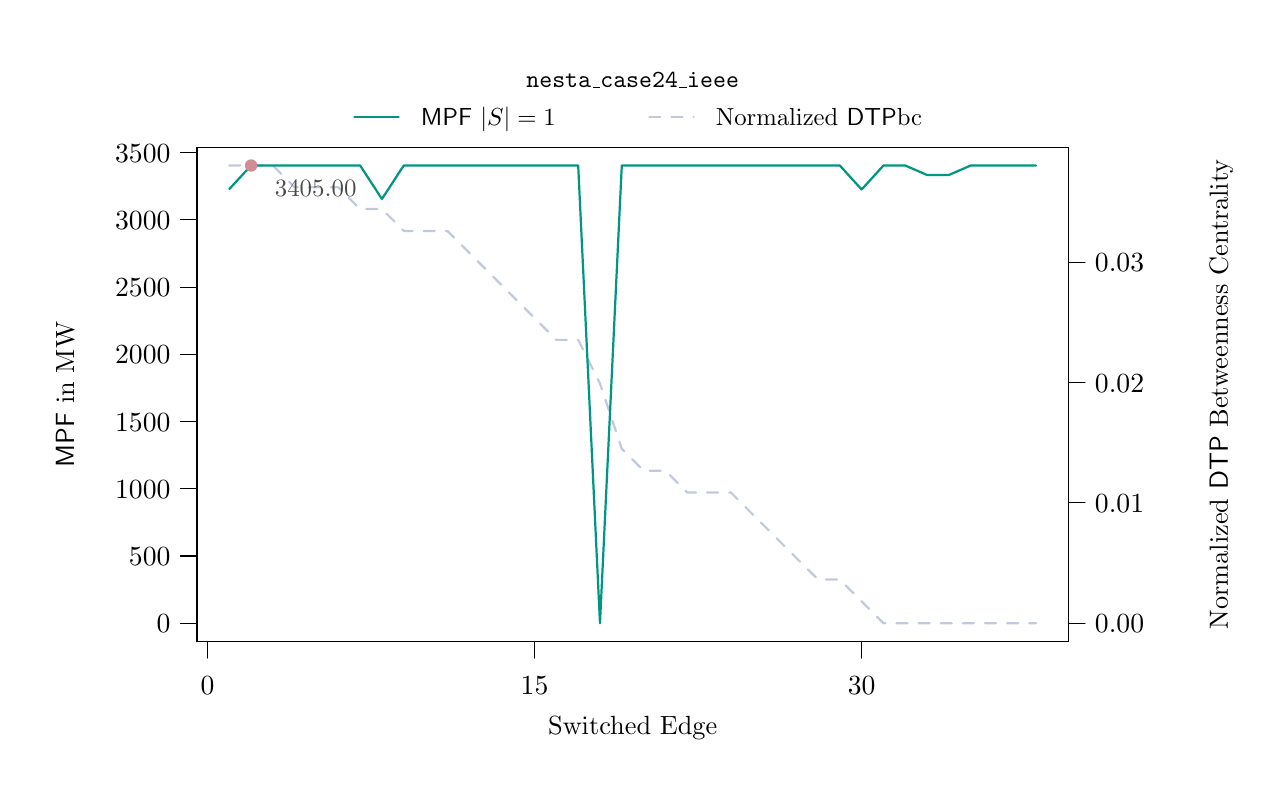
\begin{tikzpicture}[x=1pt,y=1pt]
\definecolor{fillColor}{RGB}{255,255,255}
\path[use as bounding box,fill=fillColor,fill opacity=0.00] (0,0) rectangle (440.85,271.01);
\begin{scope}
\path[clip] (  0.00,  0.00) rectangle (440.85,271.01);
\definecolor{drawColor}{RGB}{193,202,220}

\path[draw=drawColor,line width= 0.8pt,dash pattern=on 4pt off 4pt ,line join=round,line cap=round] ( 72.86,221.20) --
	( 80.74,221.20) --
	( 88.62,221.20) --
	( 96.50,213.32) --
	(104.38,213.32) --
	(112.26,213.32) --
	(120.14,205.45) --
	(128.01,205.45) --
	(135.89,197.57) --
	(143.77,197.57) --
	(151.65,197.57) --
	(159.53,189.70) --
	(167.41,181.82) --
	(175.29,173.95) --
	(183.17,166.07) --
	(191.05,158.19) --
	(198.93,158.19) --
	(206.80,142.44) --
	(214.68,118.82) --
	(222.56,110.94) --
	(230.44,110.94) --
	(238.32,103.07) --
	(246.20,103.07) --
	(254.08,103.07) --
	(261.96, 95.19) --
	(269.84, 87.32) --
	(277.72, 79.44) --
	(285.60, 71.57) --
	(293.47, 71.57) --
	(301.35, 63.69) --
	(309.23, 55.82) --
	(317.11, 55.82) --
	(324.99, 55.82) --
	(332.87, 55.82) --
	(340.75, 55.82) --
	(348.63, 55.82) --
	(356.51, 55.82) --
	(364.39, 55.82);
\end{scope}
\begin{scope}
\path[clip] (  0.00,  0.00) rectangle (440.85,271.01);
\definecolor{drawColor}{RGB}{0,0,0}

\path[draw=drawColor,line width= 0.4pt,line join=round,line cap=round] ( 61.20, 49.20) --
	(376.05, 49.20) --
	(376.05,227.81) --
	( 61.20,227.81) --
	( 61.20, 49.20);
\end{scope}
\begin{scope}
\path[clip] (  0.00,  0.00) rectangle (440.85,271.01);
\definecolor{drawColor}{RGB}{0,0,0}

\path[draw=drawColor,line width= 0.4pt,line join=round,line cap=round] (376.05, 55.82) -- (376.05,186.23);

\path[draw=drawColor,line width= 0.4pt,line join=round,line cap=round] (376.05, 55.82) -- (382.05, 55.82);

\path[draw=drawColor,line width= 0.4pt,line join=round,line cap=round] (376.05, 99.29) -- (382.05, 99.29);

\path[draw=drawColor,line width= 0.4pt,line join=round,line cap=round] (376.05,142.76) -- (382.05,142.76);

\path[draw=drawColor,line width= 0.4pt,line join=round,line cap=round] (376.05,186.23) -- (382.05,186.23);

\node[text=drawColor,anchor=base west,inner sep=0pt, outer sep=0pt, scale=  1.00] at (385.65, 52.37) {0.00};

\node[text=drawColor,anchor=base west,inner sep=0pt, outer sep=0pt, scale=  1.00] at (385.65, 95.84) {0.01};

\node[text=drawColor,anchor=base west,inner sep=0pt, outer sep=0pt, scale=  1.00] at (385.65,139.32) {0.02};

\node[text=drawColor,anchor=base west,inner sep=0pt, outer sep=0pt, scale=  1.00] at (385.65,182.79) {0.03};
\end{scope}
\begin{scope}
\path[clip] (  0.00,  0.00) rectangle (440.85,271.01);
\definecolor{drawColor}{RGB}{0,150,130}

\path[draw=drawColor,line width= 0.8pt,line join=round,line cap=round] ( 72.86,212.70) --
	( 80.74,221.20) --
	( 88.62,221.20) --
	( 96.50,221.20) --
	(104.38,221.20) --
	(112.26,221.20) --
	(120.14,221.20) --
	(128.01,209.10) --
	(135.89,221.20) --
	(143.77,221.20) --
	(151.65,221.20) --
	(159.53,221.20) --
	(167.41,221.20) --
	(175.29,221.20) --
	(183.17,221.20) --
	(191.05,221.20) --
	(198.93,221.20) --
	(206.80, 55.82) --
	(214.68,221.20) --
	(222.56,221.20) --
	(230.44,221.20) --
	(238.32,221.20) --
	(246.20,221.20) --
	(254.08,221.20) --
	(261.96,221.20) --
	(269.84,221.20) --
	(277.72,221.20) --
	(285.60,221.20) --
	(293.47,221.20) --
	(301.35,212.53) --
	(309.23,221.20) --
	(317.11,221.20) --
	(324.99,217.78) --
	(332.87,217.78) --
	(340.75,221.20) --
	(348.63,221.20) --
	(356.51,221.20) --
	(364.39,221.20);
\end{scope}
\begin{scope}
\path[clip] (  0.00,  0.00) rectangle (440.85,271.01);
\definecolor{drawColor}{RGB}{0,0,0}

\path[draw=drawColor,line width= 0.4pt,line join=round,line cap=round] ( 61.20, 49.20) --
	(376.05, 49.20) --
	(376.05,227.81) --
	( 61.20,227.81) --
	( 61.20, 49.20);
\end{scope}
\begin{scope}
\path[clip] (  0.00,  0.00) rectangle (440.85,271.01);
\definecolor{drawColor}{RGB}{0,0,0}

\path[draw=drawColor,line width= 0.4pt,line join=round,line cap=round] ( 61.20, 55.82) -- ( 61.20,225.81);

\path[draw=drawColor,line width= 0.4pt,line join=round,line cap=round] ( 61.20, 55.82) -- ( 55.20, 55.82);

\path[draw=drawColor,line width= 0.4pt,line join=round,line cap=round] ( 61.20, 80.10) -- ( 55.20, 80.10);

\path[draw=drawColor,line width= 0.4pt,line join=round,line cap=round] ( 61.20,104.39) -- ( 55.20,104.39);

\path[draw=drawColor,line width= 0.4pt,line join=round,line cap=round] ( 61.20,128.67) -- ( 55.20,128.67);

\path[draw=drawColor,line width= 0.4pt,line join=round,line cap=round] ( 61.20,152.96) -- ( 55.20,152.96);

\path[draw=drawColor,line width= 0.4pt,line join=round,line cap=round] ( 61.20,177.24) -- ( 55.20,177.24);

\path[draw=drawColor,line width= 0.4pt,line join=round,line cap=round] ( 61.20,201.53) -- ( 55.20,201.53);

\path[draw=drawColor,line width= 0.4pt,line join=round,line cap=round] ( 61.20,225.81) -- ( 55.20,225.81);

\node[text=drawColor,anchor=base east,inner sep=0pt, outer sep=0pt, scale=  1.00] at ( 51.60, 52.37) {0};

\node[text=drawColor,anchor=base east,inner sep=0pt, outer sep=0pt, scale=  1.00] at ( 51.60, 76.66) {500};

\node[text=drawColor,anchor=base east,inner sep=0pt, outer sep=0pt, scale=  1.00] at ( 51.60,100.94) {1000};

\node[text=drawColor,anchor=base east,inner sep=0pt, outer sep=0pt, scale=  1.00] at ( 51.60,125.23) {1500};

\node[text=drawColor,anchor=base east,inner sep=0pt, outer sep=0pt, scale=  1.00] at ( 51.60,149.51) {2000};

\node[text=drawColor,anchor=base east,inner sep=0pt, outer sep=0pt, scale=  1.00] at ( 51.60,173.80) {2500};

\node[text=drawColor,anchor=base east,inner sep=0pt, outer sep=0pt, scale=  1.00] at ( 51.60,198.08) {3000};

\node[text=drawColor,anchor=base east,inner sep=0pt, outer sep=0pt, scale=  1.00] at ( 51.60,222.37) {3500};
\end{scope}
\begin{scope}
\path[clip] (  0.00,  0.00) rectangle (440.85,271.01);
\definecolor{fillColor}{RGB}{207,142,147}

\path[fill=fillColor] ( 80.74,221.20) circle (  2.25);
\end{scope}
\begin{scope}
\path[clip] (  0.00,  0.00) rectangle (440.85,271.01);
\definecolor{drawColor}{RGB}{0,0,0}

\path[draw=drawColor,line width= 0.4pt,line join=round,line cap=round] ( 61.20, 49.20) --
	(376.05, 49.20) --
	(376.05,227.81) --
	( 61.20,227.81) --
	( 61.20, 49.20);
\end{scope}
\begin{scope}
\path[clip] (  0.00,  0.00) rectangle (440.85,271.01);
\definecolor{drawColor}{gray}{0.30}

\node[text=drawColor,anchor=base,inner sep=0pt, outer sep=0pt, scale=  0.90] at (104.06,210.04) {3405.00};
\end{scope}
\begin{scope}
\path[clip] (  0.00,  0.00) rectangle (440.85,271.01);
\definecolor{drawColor}{RGB}{0,0,0}

\path[draw=drawColor,line width= 0.4pt,line join=round,line cap=round] ( 64.98, 49.20) -- (301.35, 49.20);

\path[draw=drawColor,line width= 0.4pt,line join=round,line cap=round] ( 64.98, 49.20) -- ( 64.98, 43.20);

\path[draw=drawColor,line width= 0.4pt,line join=round,line cap=round] (183.17, 49.20) -- (183.17, 43.20);

\path[draw=drawColor,line width= 0.4pt,line join=round,line cap=round] (301.35, 49.20) -- (301.35, 43.20);

\node[text=drawColor,anchor=base,inner sep=0pt, outer sep=0pt, scale=  1.00] at ( 64.98, 30.00) {0};

\node[text=drawColor,anchor=base,inner sep=0pt, outer sep=0pt, scale=  1.00] at (183.17, 30.00) {15};

\node[text=drawColor,anchor=base,inner sep=0pt, outer sep=0pt, scale=  1.00] at (301.35, 30.00) {30};

\node[text=drawColor,anchor=base,inner sep=0pt, outer sep=0pt, scale=  0.95] at (218.62, 15.60) {Switched Edge};

\node[text=drawColor,rotate= 90.00,anchor=base,inner sep=0pt, outer sep=0pt, scale=  0.95] at ( 16.80,138.51) {$\mathsf{MPF}$ in~$\mathrm{MW}$};

\node[text=drawColor,rotate= 90.00,anchor=base,inner sep=0pt, outer sep=0pt, scale=  0.95] at (433.65,138.51) {Normalized~$\mathsf{DTP}$ Betweenness Centrality};
\end{scope}
\begin{scope}
\path[clip] (  0.00,  0.00) rectangle (440.85,271.01);
\definecolor{drawColor}{RGB}{0,150,130}

\path[draw=drawColor,line width= 0.8pt,line join=round,line cap=round] (118.04,238.60) -- (134.06,238.60);
\definecolor{drawColor}{RGB}{193,202,220}

\path[draw=drawColor,line width= 0.8pt,dash pattern=on 4pt off 4pt ,line join=round,line cap=round] (224.63,238.60) -- (240.65,238.60);
\definecolor{drawColor}{RGB}{0,0,0}

\node[text=drawColor,anchor=base,inner sep=0pt, outer sep=0pt, scale=  0.89] at (218.62,249.28) {\texttt{nesta\_case24\_ieee}};

\node[text=drawColor,anchor=base west,inner sep=0pt, outer sep=0pt, scale=  0.89] at (142.07,235.54) {$\mathsf{MPF}~|S|=1$};

\node[text=drawColor,anchor=base west,inner sep=0pt, outer sep=0pt, scale=  0.89] at (248.66,235.54) {Normalized~$\mathsf{DTP}$bc};
\end{scope}
\end{tikzpicture}
